% Created 2012-09-12 Wed 17:10
\documentclass[11pt]{article}
\usepackage[utf8]{inputenc}
\usepackage{fixltx2e}
\usepackage{url}
\usepackage{graphicx}
\usepackage{minted}
\usepackage{color}
\usepackage{longtable}
\usepackage{float}
\usepackage{wrapfig}
\usepackage{soul}
\usepackage{textcomp}
\usepackage{amsmath}
\usepackage{marvosym}
\usepackage{wasysym}
\usepackage{latexsym}
\usepackage{amssymb}
\usepackage[linktocpage,
  pdfstartview=FitH,
  colorlinks,
  linkcolor=blue,
  anchorcolor=blue,
  citecolor=blue,
  filecolor=blue,
  menucolor=blue,
  urlcolor=blue]{hyperref}
\usepackage{attachfile}
\tolerance=1000
\providecommand{\alert}[1]{\textbf{#1}}

\title{Molecular Simulation HOMEWORK 2: Properties of nitromethane}
\author{Zhongnan Xu}
\date{9/18/12 Thursday}
\hypersetup{
  pdfkeywords={},
  pdfsubject={},
  pdfcreator={Emacs Org-mode version 7.8.11}}

\begin{document}

\maketitle

\setcounter{tocdepth}{3}
\tableofcontents
\vspace*{1cm}

\section{Molecular Weight}
\label{sec-1}

Use ase and python to compute the molecular weight of nitromethane (CH3NO2).
Compare your answer to what you compute by hand


\begin{minted}[frame=lines,fontsize=\scriptsize,linenos]{python}
from ase.data.molecules import molecule
import numpy as np

# Calculate using ase and numpy functions
atoms = molecule('CH3NO2')
masses = atoms.get_masses()
total = masses.sum()
print 'ASE and numpy calculates the  molecular weight of nitromethane is {0:1.3f} g/mol'.format(total) 

# Calculate 'by hand' using periodic table
C = 12.011
H = 1.008
N = 14.007
O = 15.999

total = C + 3*H + N + 2*O
print 'We calculate "by hand" the molecular weight of nitromethane to be {0:1.3f} g/mol'.format(total)
\end{minted}

\begin{verbatim}
 ASE and numpy calculates the  molecular weight of nitromethane is 61.040 g/mol
 We calculate "by hand" the molecular weight of nitromethane to be 61.040 g/mol
\end{verbatim}
\section{Center of Mass}
\label{sec-2}

The center of mass is defined as 
\begin{equation}
R = \frac{1}{M} \sum m_ir_i
\end{equation}
where $M$ is the total mass and $m_i$ and $r_i$ is each chemical species' mass
and distance from a fixed point. Note that $R$ and $r_i$ are given from the same
fixed point, which we will define for simplicity as the origin. We will first write
a program that calculates this.


\begin{minted}[frame=lines,fontsize=\scriptsize,linenos]{python}
from ase.data.molecules import molecule
import numpy as np

# Prepare the data
atoms = molecule('CH3NO2')
masses = atoms.get_masses()
positions = atoms.get_positions()
total_mass = masses.sum()

# Compute the center of mass (COM). First compute the sums of the m*r values
sum = np.array((0., 0., 0.))
for mass, pos in zip(masses, positions):
    sum += mass * pos
COM = sum / total_mass
print 'We compute the center of mass to be ({0:1.5f}, {1:1.5f}, {2:1.5f})'.format(COM[0], COM[1], COM[2])

# Use ASE to compute the center of mass
COM = atoms.get_center_of_mass()
print 'ASE computes the center of mass to be ({0:1.5f}, {1:1.5f}, {2:1.5f})'.format(COM[0], COM[1], COM[2])
\end{minted}

\begin{verbatim}
 We compute the center of mass to be (0.00619, 0.07989, 0.00000)
 ASE computes the center of mass to be (0.00619, 0.07989, 0.00000)
\end{verbatim}
\section{Moments of Inertia}
\label{sec-3}


\begin{minted}[frame=lines,fontsize=\scriptsize,linenos]{python}
from ase.data.molecules import molecule
atoms = molecule('CH3NO2')
I = atoms.get_moments_of_inertia()
print 'The moments of inertia are {0:1.3f}, {1:1.3f}, and {2:1.3f} amu*angstroms^2'.format(I[0], I[1], I[2])
\end{minted}

\begin{verbatim}
 The moments of inertia are 42.242, 47.838, and 86.868 amu*angstroms^2
\end{verbatim}
\section{Bond Lengths}
\label{sec-4}


\begin{minted}[frame=lines,fontsize=\scriptsize,linenos]{python}
from ase.data.molecules import molecule

atoms = molecule('CH3NO2')
print 'atom symbol'
print '==========='
for i, atom in enumerate(atoms):
    print i, '   ' + atom.symbol

# From here we need to find distances between atom indexes 0-2, 0-3, and 0-4
indexes = ((0, 2), (0, 3), (0, 4))
print 'The C-H bond distances are'
for index in indexes:
    print '{0:1.3f}'.format(atoms.get_distance(index[0], index[1])), 'Angstroms'
\end{minted}


\begin{verbatim}
atom symbol
===========
0    C
1    N
2    H
3    H
4    H
5    O
6    O
The C-H bond distances are
1.090 Angstroms
1.087 Angstroms
1.087 Angstroms
\end{verbatim}

To understand why they are not equal, we can look at the molecule.


\begin{minted}[frame=lines,fontsize=\scriptsize,linenos]{python}
from ase.data.molecules import molecule
from ase.visualize import view
from ase.io import write

atoms = molecule('CH3NO2')
atoms.set_cell((10, 10, 10))
atoms.center()
write('CH3NO2.png', atoms, show_unit_cell=2)
write('CH3NO2_rot.png', atoms, show_unit_cell=2, rotation='-90x,-90y, 90z')
\end{minted}


\begin{figure}[H]
\centering
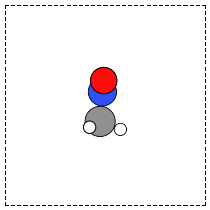
\includegraphics[width=0.7\textwidth]{./CH3NO2.png}
\caption{Side view of CH$_{\mathrm{3NO}}$$_2$}
\end{figure}
\begin{figure}[H]
\centering
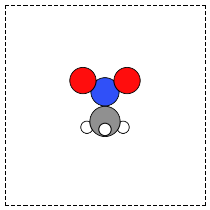
\includegraphics[width=0.7\textwidth]{./CH3NO2_rot.png}
\caption{Side view of CH$_{\mathrm{3NO}}$$_2$}
\end{figure}

We can see that the molecule is symmetric along a plane that splites the
two oxygens. These therefore will have the same bond length.
\section{Bond angle in the nitro group}
\label{sec-5}

From the previous problem, we know the indexes of the O-N-O bond are 6, 1, and 5


\begin{minted}[frame=lines,fontsize=\scriptsize,linenos]{python}
from ase.data.molecules import molecule
from numpy import pi

atoms = molecule('CH3NO2')
s = 'The angle between O-N-O is {0:1.1f} degrees'
print s.format(atoms.get_angle([6,1,5])*180/pi)
\end{minted}

\begin{verbatim}
 The angle between O-N-O is 125.7 degrees
\end{verbatim}
\section{Generate an xyz file}
\label{sec-6}


\begin{minted}[frame=lines,fontsize=\scriptsize,linenos]{python}
from ase.data.molecules import molecule
from ase.io import write

atoms = molecule('CH3NO2')
write('CH3NO2.xyz', atoms)
file = open('CH3NO2.xyz', 'r')
lines = file.readlines()
for line in lines:
    print line[0:-1] #We want this to avoid the extra new line at the end of each line
\end{minted}

\begin{verbatim}
 7
 
 C      -0.114282000000000     -1.314565000000000      0.000000000000000
 N       0.000000000000000      0.166480000000000      0.000000000000000
 H       0.899565000000000     -1.715256000000000      0.000000000000000
 H      -0.640921000000000     -1.607212000000000      0.904956000000000
 H      -0.640921000000000     -1.607212000000000     -0.904956000000000
 O       0.066748000000000      0.728232000000000     -1.103775000000000
 O       0.066748000000000      0.728232000000000      1.103775000000000
\end{verbatim}
\section{Create a graphic of nitromethane}
\label{sec-7}


\begin{minted}[frame=lines,fontsize=\scriptsize,linenos]{python}
from ase.data.molecules import molecule
from ase.visualize import view
from ase.io import write

atoms = molecule('CH3NO2')
atoms.set_cell((10, 11.5, 12.1))
atoms.center()
write('CH3NO2_image.png', atoms, show_unit_cell=2, rotation='-45x,-45y, 45z')
\end{minted}

\begin{figure}[H]
\centering
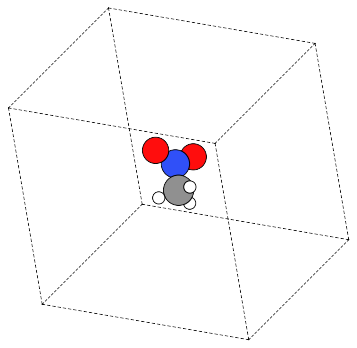
\includegraphics[width=0.7\textwidth]{./CH3NO2_image.png}
\caption{Graphic of nitromethane}
\end{figure}

\end{document}
